\section{Smart Street Sensor Project}

The Smart Street Sensor project is one of the most comprehensive study carried out on consumer volume and characteristics in retail areas across UK.
The project has been organised as a collaboration between Local Data Company (LDC) and Consumer Data Research Centre,  University College London (CDRC, UCL).
The data for the study is generated independently within the project through sensors installed at around 1000 locations across UK.
When completed, the project will serve as the first and unique comprehensive research into the patterns of retail activity in UK high streets.

The primary aim of the project is to improve our understanding of the dynamics of the high street retail in UK.
As we saw in our literature search, unlike online retail, this involves quantification and measurement of human activity at small scales, such as high streets which already the subject of active research.
The key challenge in this area is the collection of data at smallest scales possible with minimal resources while not infringing on people’s privacy.
This challenge when solved can provide immense value to occupiers, landlords, local authorities, investors and consumers within the retail industry.
The project aims to facilitate decision making by stakeholders in addition to the tremendous opportunities for academic research.

\subsection{Methodology}

\begin{marginfigure}[2cm]
  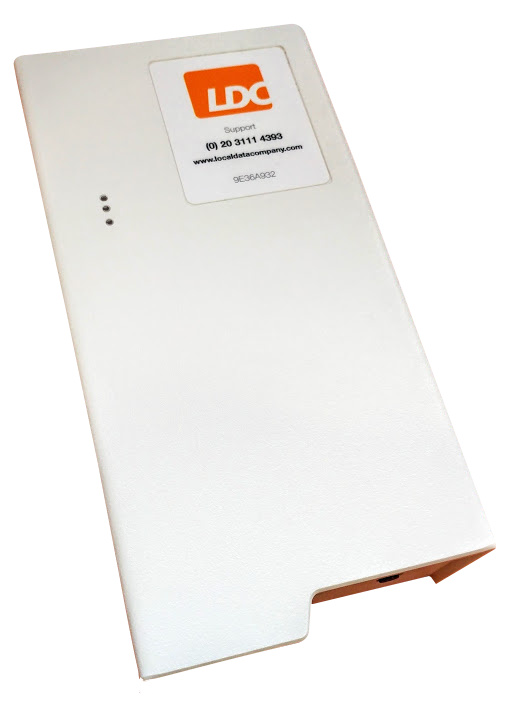
\includegraphics{images/sss-hardware.jpg}
  \caption{Hardware setup used to collect data in the pilot studies.}
  \label{figure:collection:pilot:hardware}
\end{marginfigure}


As a first step, various locations for the study were identified by CDRC to include a wide geographical spread, different demographic characteristics and range of retail centre profiles.
A custom footfall counting technology using WiFi based sensors was also designed, developed by LDC and the sensors were installed the identified locations.
The sensor monitors and records signals sent by WiFi enabled mobile devices present in its range.
In addition, the number of people walking by the sensor was counted manually for short time periods during the installation.
The project aims to combine these two sets of data to use as a proxy for estimating footfall at these locations.
The potentially identifiable information collected on the mobile devices is hashed at sensor level and the data is sent to central server via encrypted channel for storage.
This data is then retrieved securely for the preparation of the commercial dashboards by LDC and for research purposes by CDRC users.
The project began on July 2015 with the first sensor installation and has grown to an average of 450 daily active sensors as of January 2017.

The data is collected through set of SmartStreetSensors (shown in Figure 3.1), a WiFi based sensor which when installed acts as a WiFi access point and collects specific type of packets (probe requests) relayed by mobile devices which are which are within the device’s signal range and are searching for available access points.
The sensor is usually installed on partnering retailer's shop windows so that its range covers the pavement in front of the shops.
The installation and calibration of device with respect to the shop window and the pavement is illustrated in Figure 3.2.
There is also a small percentage (3\%) of the devices which are installed within large shops to monitor internal footfall.
Each device collects data independently and uploads the collected data to a central container at regular interval 5 minutes through a dedicated 3G mobile data connection.
The sensor hardware has been improved over the course of the project and currently has built in failure prevention mechanisms such as, backup battery for power failures, automatic reboot capabilities and in-device memory for holding data when internet is not available.
The hardware versions and the corresponding features are detailed in Table 3.1.

\begin{figure*}
  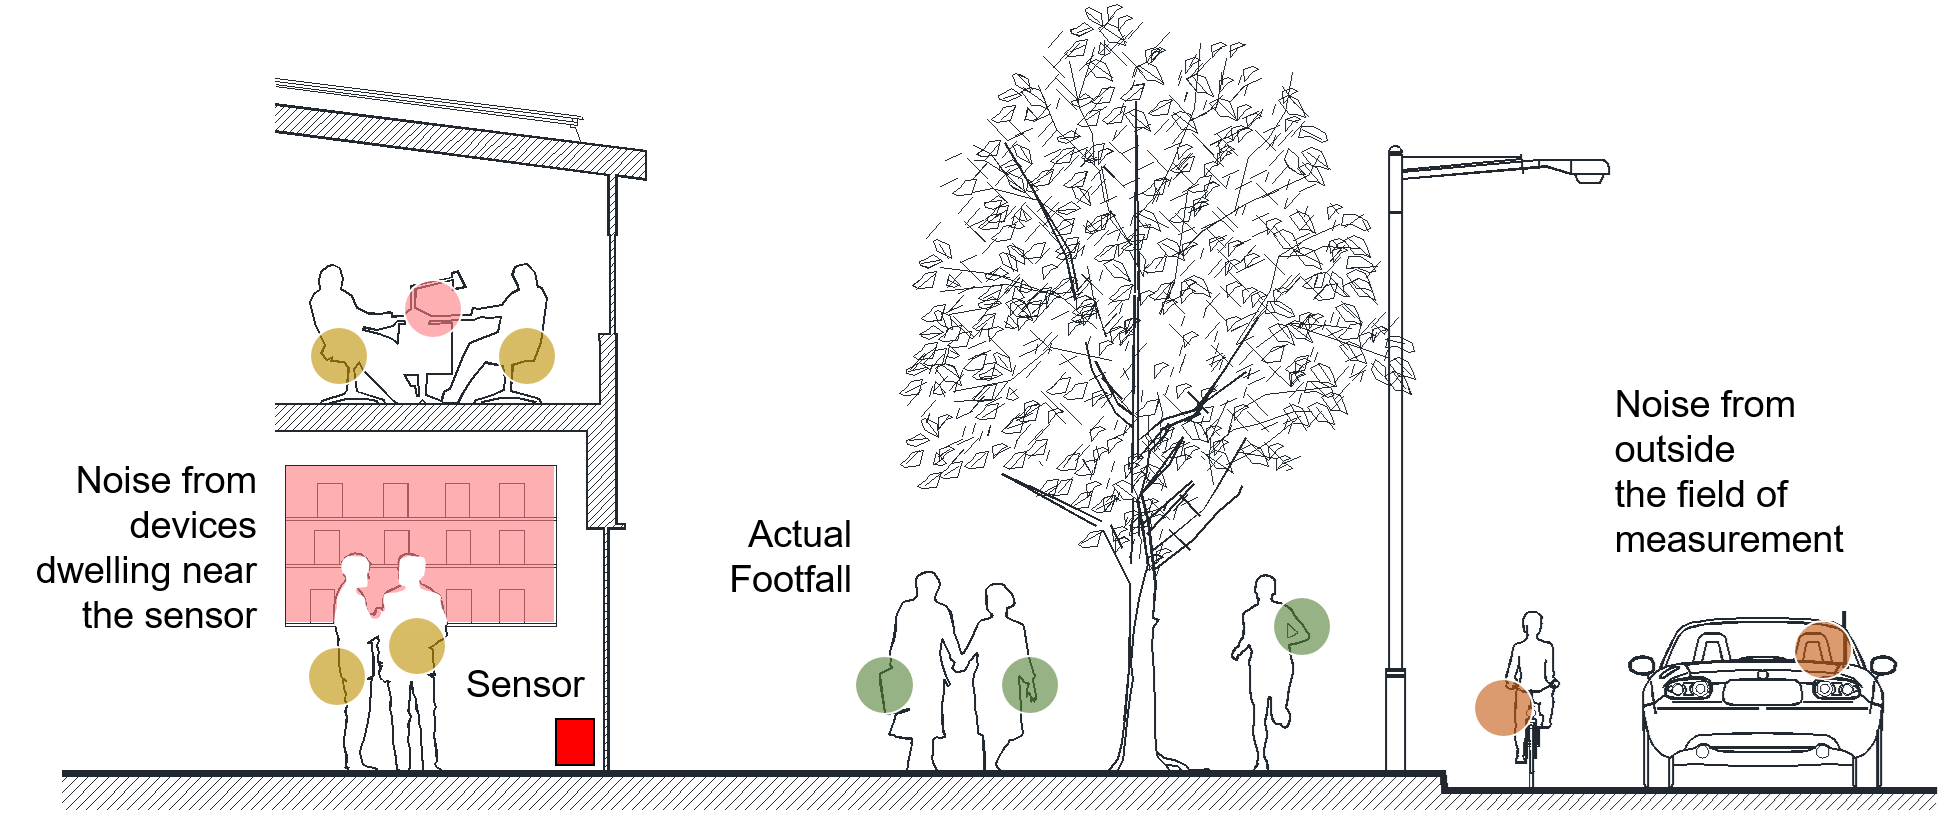
\includegraphics{images/sss.png}
  \caption{Outline of the `Medium data toolkit' devised to collect, process, visualise and manage the Wi-Fi probe requests data}
  \label{figure:literature:tech:timeline}
\end{figure*}

\lipsum[1-2]

%+200 words
system architecture - figure.

\subsection{Locations}
%(300 words)
\begin{marginfigure}[8cm]
  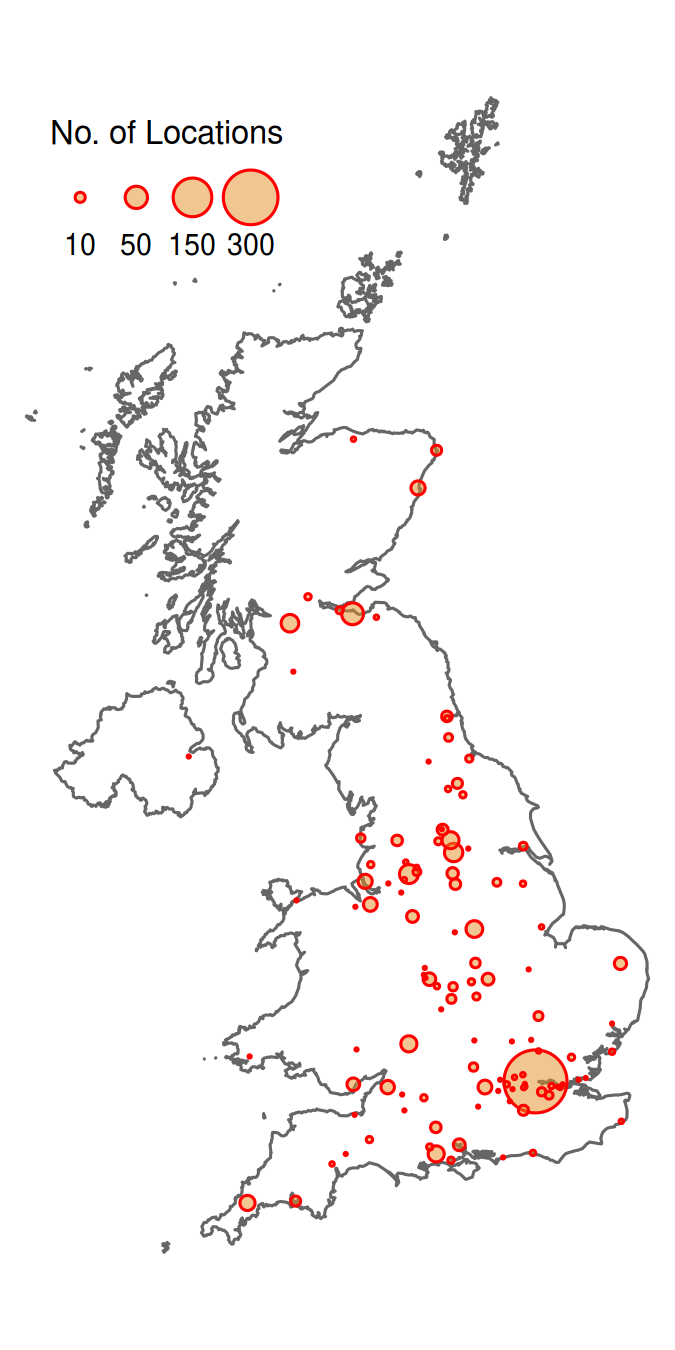
\includegraphics[trim = {0 20 0 0}, clip]{images/sss-locations.png}
  \caption{Outline of the `Medium data toolkit' devised to collect, process, visualise and manage the Wi-Fi probe requests data}
  \label{figure:literature:tech:timeline}
\end{marginfigure}

\lipsum[1]
locations - table

\subsection{Data Description}

% data description - table.
% sample probe request - code.
% installation of sensors - figure.
% descriptive statistics - table.

\lipsum[1-3]



\pagebreak

